\subsection{Storing and Ingesting the Data}
In this section we will discuss which data storage solution we are going to use and why. We will compare a few options and select the best. We will then briefly explain how it works and how we plan to use it.

\subsubsection{Storing Extracted Categories}
The categories that are extracted from documents, as described in the previous section, need to be stored. We want to be able to apply different models on the data and we also want access to the raw data. \\
To keep this flexibility and to maintain scalability, we save the document information in conjunction with the category. The documents that are deemed useful are stored on disk, pointed to by the document information node. Occurrences of cities in a document are stored as a relation of these cities to the document. This means that if a relation "transportation" is extracted from a document that contains the cities "Rotterdam" and "Amsterdam", we create an document node and create relations from Amsterdam to the node and from Rotterdam to the node. In the end, when all documents have been stored and relations created, the relation between two cities can be computed by counting document in which they both appear, grouping by category. \\
Considering the fact that relations are bidirectional, meaning a relation of "Transportation" between "Rotterdam-Amsterdam" implicates a relation of "Transportation" between "Amsterdam-Rotterdam" as well, we only need one relation between two distinct cities.

\subsubsection{Graph Database or Traditional Database}
To store the relationships and documents discussed in the previous subsection, there are two possibilities: (1) graph databases and (2) traditional relational databases.

Because visualisation of the network of cities as a graph is an important part of the application, and relations between cities play a key role in the system, we need a database that is designed for these features. Relations are the most important in the graph data model, where this is not true for traditional relational databases. Vicknair et al. stated that a graph database such as Neo4j has an easily mutable schema, where a relational database schema is less mutable \cite{vicknair2010}. Furthermore, the edges between nodes in a graph database can have properties, which is exactly what the envisioned data structure should be for this application. Lastly, if the desire arises to find indirect relationships between cities then a graph database is most appropriate choice. For example, if the client wishes to find out how Alkmaar is connected to Tokyo via other cities then the need for fast graph traversal arises. According to the graph database Neo4j their graph traversal is already 60\% faster than a relational database for a depth of just 3\footnote{\url{https://neo4j.com/news/how-much-faster-is-a-graph-database-really/}}.  Therefore, we are confident that a graph database is the best choice.

\subsubsection{Comparing Graph Databases}
Next, the type of database needs to be selected. For this, six of the most popular databases according to the solid IT Graph DBMS ranking\footnote{\url{https://db-engines.com/en/ranking/graph+dbms}\label{ranking}}.  This rating is established using multiple parameters, among these parameters is the number of mentions on websites and in job offers. Next to that, the parameters also include the number of searches, relevance in social networks and the general interest in the system\footnote{\url{https://db-engines.com/en/ranking_definition}}. These six most popular Graph Databases are rated on five important aspects. These are, is the graph database open-source, scalable, free, does it support Python and has built-in visualisation. Open-source is important because the application should be as transparent as possible to achieve maximum credibility, therefore it helps that the graph database is open-source. A scalable database is necessary to achieve the design goal \"scalable\". Next to that, a free graph database is preferred so we won't leave the client with costs to keep the application running. The Python and Built-in visualisation aspects are important for fast development, as built-in visualisation allows visualising the data before building a front-end for the application.


\noindent\begin{threeparttable}
\begin{tabular}{@{} l *5c @{}}    \toprule
\emph{name} & \emph{Open-source} & \emph{Scalable} & \emph{Python support} & \emph{Free} & \emph{Built-in Visualisation}\\  \\\midrule
AllegroGraph    & \XSolidBrush  & \Checkmark  & \Checkmark  & \Checkmark\tnote{a} & \XSolidBrush\tnote{b} \\ 
ArangoDB  & \Checkmark & \Checkmark & \Checkmark & \Checkmark & \Checkmark\\ 
Neo4j  & \Checkmark & \Checkmark & \Checkmark & \Checkmark\tnote{c} & \Checkmark\\ 
OrientDB  & \Checkmark & \Checkmark & \Checkmark & \Checkmark & \Checkmark\\ 
Teradata Aster & \XSolidBrush & \Checkmark & \Checkmark & \XSolidBrush & \XSolidBrush\tnote{d}\\ 
Titan  & \Checkmark & \Checkmark & \XSolidBrush & \Checkmark & \XSolidBrush\tnote{e}\\\bottomrule
 \hline
\end{tabular}
\begin{tablenotes}
\item[a] Only free up to 5 million triples
\item[b] With separate tool called Gruff: \url{https://allegrograph.com/gruff2/}
\item[c] Non-commercial use
\item[d] Using a separate tool Aster AppCenter
\item[e] Using a separate tool 
\end{tablenotes}
\end{threeparttable}\\

From this table, it can be deduced that three of these graph databases are viable candidates: ArangoDB, Neo4j and OrientDB. For this project, Neo4j is the best choice because of three reasons. Firstly because we have experience with Neo4j, which means less time will be spent on getting to know the graph database and functionality. Secondly because it is by far the most popular graph database $^{\ref{ranking}}$. Thirdly, since Neo4j is the most popular graph database, the support community and amount of available examples is large.

\subsubsection{Using Neo4j for Storage and Ingestion}
Neo4j is a highly scalable native graph database that leverages data relationships as first-class entities \cite{neo4j}. It is the single highly scalable, fast and ACID compliant graph database available. ACID stands for the four properties atomicity, consistency, isolation and durability of transactions in database systems that ensure reliability for query results \cite{haerder1983principles}. The scalability of Neo4j comes from the fact that is easily spread across clusters, which provides a read throughput that scales linearly. Next to that, when spread across clusters Neo4j provides data redundancy and still high write speed \cite{neo4jscalable}. Additionally, Neo4j is free to use for non-commercial purposes. To illustrate how scalable Neo4j is, consider that very large companies such as eBay, Cisco, Walmart, HP and LinkedIn\footnote{\url{https://neo4j.com/customers/}} use it in their mission-critical systems. Holzschuher and Peinl compared the performance of Neo4j to the more classic and commonly used NoSQL databases and found that the more natural representation of relationships resulted in significant performance increase gains~\cite{holzschuher2013performance}. Jouili et al. concluded that Neo4j has a read-only performance which is comparable to other graph databases \cite{jouili2013}. Compared to other databases Neo4j is slower with writing. However, the application will eventually do more reading than writing making writing a less important aspect.

There are some specific aspects of Neo4j that make it a very suitable candidate for this application. These are:

\begin{description}
\item[properties] Any entity in the Neo4j graph can be given properties (key-value pairs) containing information about the entity. Properties are primarily meant to provide additional information and are less suitable to be queried on. As an example, a city can have a number of inhabitants and districts attached to it as a property.
\item[labels] Nodes can be tagged with a label, describing their roles in the network. These annotations are especially useful to filter the data set on one or more categories. For example, a city can be labelled as "capital" to be able to distinguish between regular and capital cities.
\item[relations] Nodes can be connected using relationships. These are always directed, typed and named and can have properties. Using these properties, one can control how the graph is traversed. For example, if a path (relationship) is to be avoided unless absolutely necessary, the relation can be given a high cost. To give importance to some relationship, one could also assign a strength score to it. Since relationships are handled efficiently by Neo4j, nodes can have any number of relationships linked to it without compromising performance. For our purpose, a relation could comprise the strength of the relationship between two cities (nodes).
\end{description}

The Neo4j model can be depicted as shown in figure \ref{fig:neo4j}. It consists of nodes, relationships (edges), properties (within the nodes) and labels (rectangular blocks above the nodes).

\begin{figure}[h]
\centering
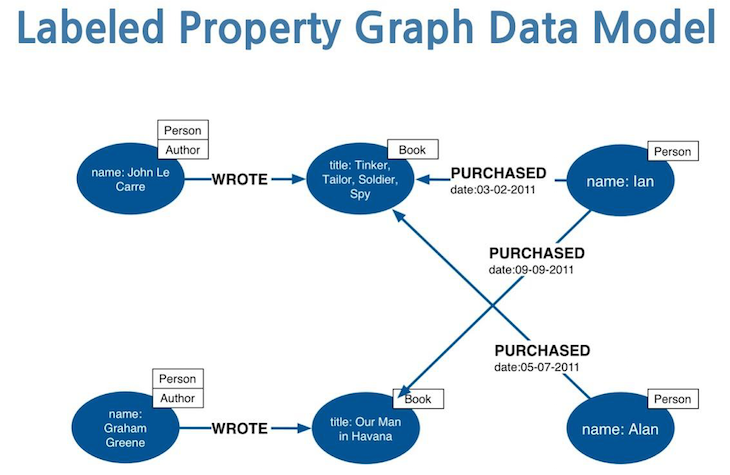
\includegraphics[width=0.75\textwidth]{neo4j}
\caption{The Neo4j model \protect\footnotemark{}}
\label{fig:neo4j}
\end{figure}
\footnotetext{\url{https://neo4j.com/developer/graph-database/}}

Besides the aforementioned useful properties of Neo4j, the graph can be put to good use for visualising the global urban network. By adding a location property to a city, nodes and relations can be mapped directly to a geographical map. Most importantly, indices of text files can be stored that mention the city as properties of nodes. That way, we are able to generate a subset of files that can be analysed for calculating the strength of the relationship between the nodes.









% --------------------------------------------Maybe useful in future----------------------------------------------------
\begin{comment}
\subsubsection{Elasticsearch}
Elasticsearch is an open-source search engine which centrally stores your data \cite{Elasticsearch}. It is a fast and scalable solution that was designed with big data search in mind. According to Kononenko et al. \cite{Kononenko2014} Elasticsearch has some significant advantages in comparison with traditional relational databases. Two of these advantages are scalability and performance. 

\paragraph{Scalability} According to Elasticsearch \cite{Elasticsearch} their product has no problem with scaling horizontally. It automatically manages indices and queries distributed across a cluster. This is an important feature as it is likely that the amount of data that our solution will use and process will increase and we do not want to keep upgrading the server that contains database, which would be vertical scalability. {\color{red} FIXME: Referentie naar dat we alleen NL doen nu? En daarom scalability nogal belangrijk is}

\paragraph{Performance}
Because Elasticsearch was designed to handle documents and perform full-text search it not surprising it performs well doing this. As we're going to be using the same kind of input data we expect Elasticsearch as the most choice. Kononenko et al. found that while scalability and schema-free documents are common for NoSQL systems, the combination of all three (scalability, agility, and performance) in one system is what makes Elasticsearch stand out from other systems. Following this, we conclude Elasticsearch would be a good choice as a data storage and search platform for our {\color{red} FIXME: solution|product|project.. (We moeten even kiezen welke we aanhouden zodat we dat overal hetzelfde doen}.\\

\paragraph{Downsides} \label{sec:elastic-downsides}
A downside of Elasticsearch is that it does not have any form of security out of the box. This means that everyone with the server address could access the data. This is not a problem for CommonCrawl data, as this was already available online anyway. However, when using for example Delpher or other sources you need a license this becomes a problem. Next to that, it would also be possible for anyone to meddle with the data in Elasticsearch making the data unreliable. Elasticsearch provides a Security package for which you unfortunately need a paid license. However, to secure Elasticsearch while making it available for users we could use a plugin such as Search Guard\footnote{\url{http://floragunn.com/searchguard/}} or use a special proxy as proposed by Kononenko et al. \cite{Kononenko2014}.

Another downside of Elasticsearch is that transactions involving multiple documents\footnote{\url{https://www.elastic.co/guide/en/elasticsearch/guide/current/concurrency-solutions.html}} are not ACIDic. Where ACID stands for the four properties atomicity, consistency, isolation and durability regarding transactions in database systems \cite{haerder1983principles}. This means that we need to keep concurrency problems in mind and will probably need to enable some locking to prevent these concurrency problems when performing transactions on multiple documents. 



\subsubsection{Hadoop}
Because we are designing a \maybe{application} that will use and parse a lot of data, it will be useful to use distributed computing. Although we only use the .nl data \maybe{Totale grootte van data noemen?} from CommonCrawl for this \todo{project} (see section \ref{sec:commoncrawl}) we could still benefit from distributed computing, especially with the future of the \maybe{application} in mind. 
Therefore we want to use Apache Hadoop, which is a framework that allows for the distributed processing of large data sets across clusters of computers using simple programming models \cite{Hadoop}. With this open source software we could distribute the computations from a single server across many more devices, thereby speeding up the process. 

\end{comment}